% Introducción

\chapter{Detección de tumores}

Link del dataset: https://www.kaggle.com/datasets/preetviradiya/brian-tumor-dataset/data

\section{Descripción del dataset}

La metadata informa que el dataset contiene 4600 imágenes en total, divididas en dos clases: $tumor$ y $normal$ según se observa en la Fig. \ref{fig.clases}. En este contexto va a entenderse a $normal$ como $sin$ $tumor$, pero no significa que no existan otras patologías por ejemplo isquemias.

\begin{figure}[H]
\centering
        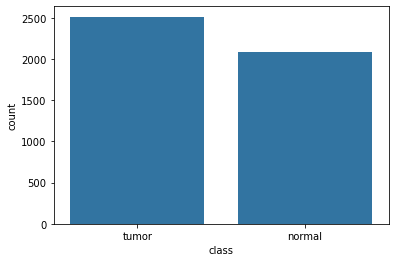
\includegraphics[width=0.5\linewidth]{chapters/deteccion/images/clases.png}
        \caption{Distribución de clases de imágenes del dataset para detección.}
        \label{fig.clases}
  \end{figure}


En la Fig. \ref{fig:conjunto_imagenes} se observan algunas imágenes del dataset. En particular, las Fig. \ref{fig:normal1}, \ref{fig:normal2} y \ref{fig:normal3} corresponden a pacientes normales mientras que las Fig. \ref{fig:tumor1}, \ref{fig:tumor2} y \ref{fig:tumor3} corresponden a pacientes con tumor cerebral. 

\begin{figure}[H]
    \centering
    \begin{subfigure}[b]{0.3\textwidth}
        \centering
        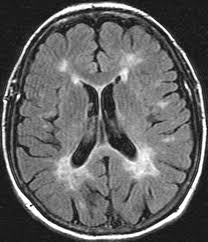
\includegraphics[width=\linewidth]{chapters/deteccion/images/sano1.jpg}
        \caption{Axial T2 flair con isquemias periventriculares. Normal.}
        \label{fig:normal1}
    \end{subfigure}
    \hfill
    \begin{subfigure}[b]{0.3\textwidth}
        \centering
        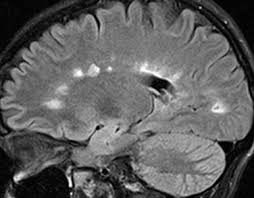
\includegraphics[width=\linewidth]{chapters/deteccion/images/sano2.jpg}
        \caption{Sagital T2 flair. Isquemias.}
        \label{fig:normal2}
    \end{subfigure}
    \hfill
    \begin{subfigure}[b]{0.3\textwidth}
        \centering
        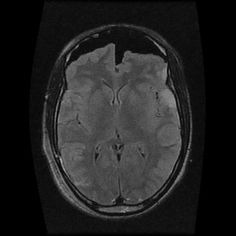
\includegraphics[width=\linewidth]{chapters/deteccion/images/sano3.jpg}
        \caption{Axial T2 flair. Normal.}
        \label{fig:normal3}
    \end{subfigure}
    
    \vspace{0.5cm}
    
    \begin{subfigure}[b]{0.3\textwidth}
        \centering
        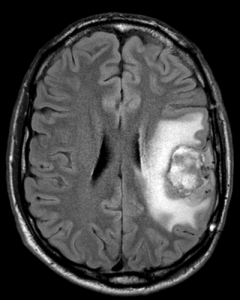
\includegraphics[width=\linewidth]{chapters/deteccion/images/cancer1.png}
        \caption{Axial T2 flair. Tumor.}
        \label{fig:tumor1}
    \end{subfigure}
    \hfill
    \begin{subfigure}[b]{0.3\textwidth}
        \centering
        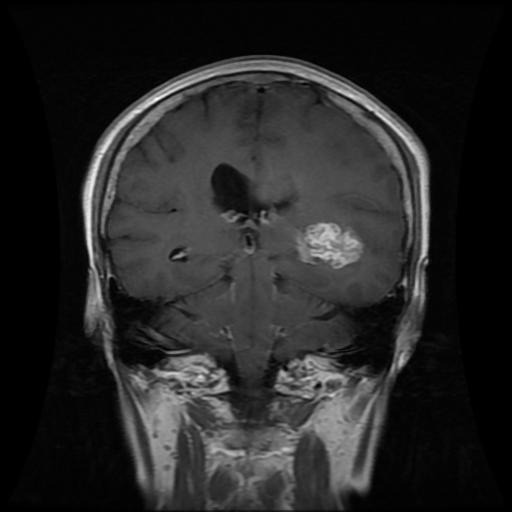
\includegraphics[width=\linewidth]{chapters/deteccion/images/cancer2.jpg}
        \caption{Coronal T1 con contraste. Tumor.}
        \label{fig:tumor2}
    \end{subfigure}
    \hfill
    \begin{subfigure}[b]{0.3\textwidth}
        \centering
        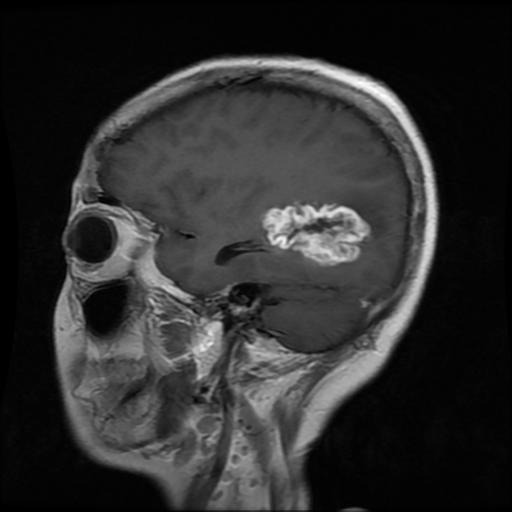
\includegraphics[width=\linewidth]{chapters/deteccion/images/cancer3.jpg}
        \caption{Sagital T1 con contraste. Tumor.}
        \label{fig:tumor3}
    \end{subfigure}
    \caption{Muestra de imágenes del dataset.}
    \label{fig:conjunto_imagenes}
\end{figure}

Es interesante notar que la Fig. \ref{fig:normal1} es un corte axial $T_2$ flair de cerebro donde claramente se observa una anormalidad del tejido. Las zonas hiperintensas (blancas) que rodean a los ventrículos de forma bilateral corresponden a isquemias típicas de la edad pero no es un tumor, por lo tanto la imagen es clasificada como de paciente sano. 

Por otro lado, una patología isquémica también se observa en la Fig. \ref{fig:tumor1}, en este caso está rodeando a un tumor. Por lo tanto, esta imagen se clasifica como tumoral. 

\section{Preprocesamiento de las imágenes}

Las imágenes disponibles tenían no solo diferentes tamaños sino también diferentes relaciones de aspecto. La Fig. \ref{fig.relaciones} muestra la distribución de tamaños, la recta roja corresponde a imágenes que sean cuadradas.

\begin{figure}[H]
\centering
        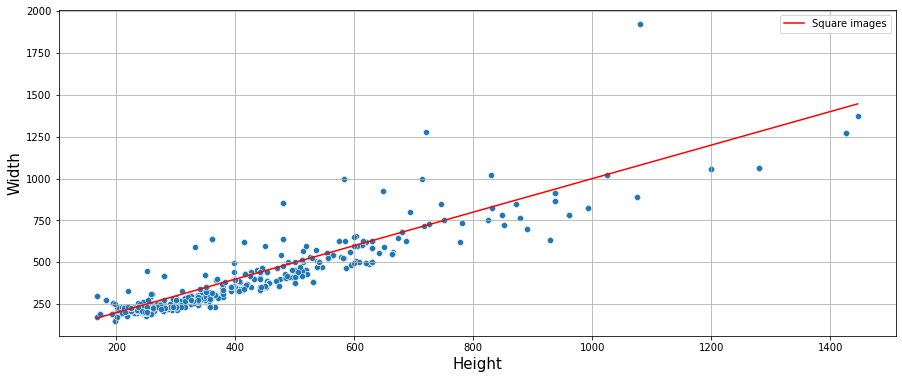
\includegraphics[width=\linewidth]{chapters/deteccion/images/relaciones.png}
        \caption{Tamaños de las imágenes del dataset}
        \label{fig.relaciones}
  \end{figure}

Con el objetivo de normalizar las imágenes, se optó por redimensionarlas a una resolución de $256 \times 256$ píxeles. 

Además, se aplicó una conversión a escala de grises, dado que esta representación es ampliamente utilizada en el ámbito del diagnóstico médico, garantizando así una compatibilidad estándar para el análisis y la interpretación de las imágenes.

Un último preprocesamiento que se aplicó es normalizar el rango de valores de los píxeles de la imagen, originalmente cada píxel $p_{ij}\in [0,255]$ y luego de la transformación $p_{ij}\in [0,1]$.

\section{Modelos}

Antes de aplicar los diferentes modelos se realizó la partición en $train/test$ en una proporción $80/20$. 

Las variables predictoras son los propios píxeles de cada imagen, mientras que el target es binario: tumor/sano. 

Inicialmente se aplicaron modelos tradicionales de $\textit{machine learning}$. Para estos modelos anteriores se realizó un preprocesamiento más, la conversión de las imágenes en formato de matriz ($256\times256$) a vector de dimensión $256\cdot256=65536$. Los modelos trabajados fueron:

\begin{itemize}
\item Naive bayes
\item Random Forest Classifier
\item Logistic Regression
\item Decision Tree Classifier
\item KNN
\end{itemize}.


\subsection{Naive bayes}

Este modelo por ser el más simple de todos constituye un baseline. Luego del entrenamiento se obtuvieron la matriz de confusión y curva roc tanto para train como para test, las cuales son mostradas en la Fig. \ref{fig.naive}. 

\begin{figure}[H]
\centering
        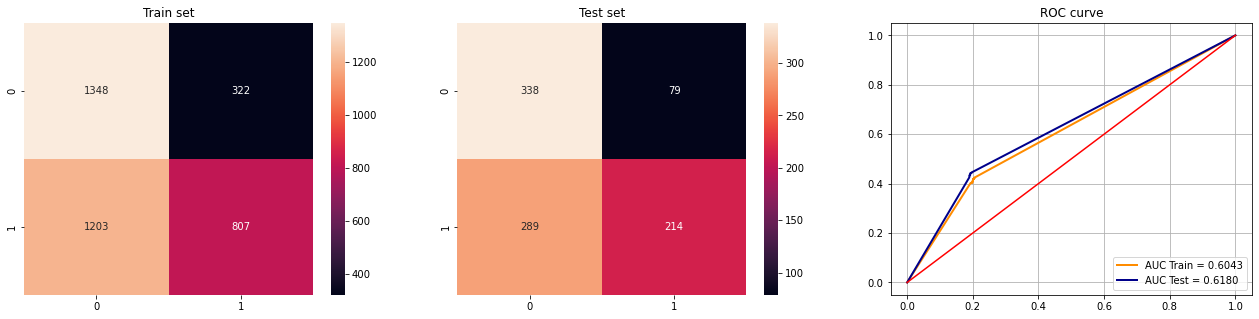
\includegraphics[width=\linewidth]{chapters/deteccion/images/naive.png}
        \caption{Métricas para el modelo Naive-Bayes}
        \label{fig.naive}
  \end{figure}
  
  En la Tabla \ref{tabla.naive} se detallan las métricas derivadas de la matriz de confusión. Se observa que las métricas son bajas, lo cual es coherente con que es un modelo demasiado simple. 

\begin{table}[H]
\centering
\begin{tabular}{|c|c|c|c|c|c|}
\hline
      & Accuracy & Precision & Recall & AUC    & $F_1$ score \\ \hline
Train & 0.5856   & 0.7148    & 0.4015 & 0.6043 & 0.5142      \\ \hline
Test  & 0.6      & 0.7304    & 0.4254 & 0.618  & 0.5377      \\ \hline
\end{tabular}
\caption{Métricas para el modelo Naive-Bayes}
\label{tabla.naive}
\end{table}

\subsection{Random forest}

Luego del entrenamiento se obtuvieron la matriz de confusión y curva roc tanto para train como para test, las cuales son mostradas en la Fig. \ref{fig.rf}. 

\begin{figure}[H]
\centering
        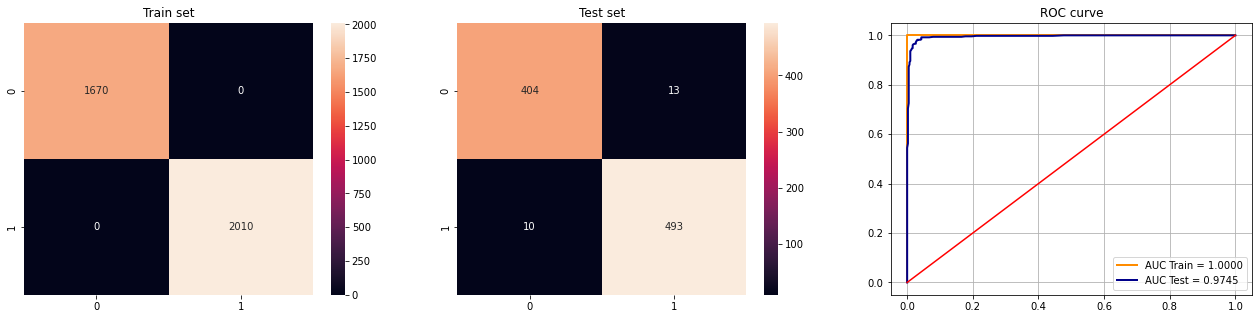
\includegraphics[width=\linewidth]{chapters/deteccion/images/rf.png}
        \caption{Métricas para el modelo Random Forest}
        \label{fig.rf}
  \end{figure}
  
 En la Tabla \ref{tabla.rf} se detallan las métricas derivadas de la matriz de confusión. Se observa que las métricas son bajas, lo cual es coherente con que es un modelo demasiado simple. 

\begin{table}[H]
\centering
\begin{tabular}{|c|c|c|c|c|c|}
\hline
      & Accuracy & Precision & Recall & AUC    & $F_1$ score \\ \hline
Train & 1.0   & 1.0    & 1.0 & 1.0 & 1.0      \\ \hline
Test  & 0.975      & 0.9743    & 0.9801 & 0.9745  & 0.9772      \\ \hline
\end{tabular}
\caption{Métricas para el modelo Random Forest}
\label{tabla.rf}
\end{table}

Es notable que este modelo resulta perfecto para el conjunto de entrenamiento, lo cual haría sospechar de un posible overfitting, pero viendo las métricas correspondientes al conjunto de test esto parecería estar descartado. 


\subsection{Logistic regression}

Luego del entrenamiento se obtuvieron la matriz de confusión y curva roc tanto para train como para test, las cuales son mostradas en la Fig. \ref{fig.lr}. 

\begin{figure}[H]
\centering
        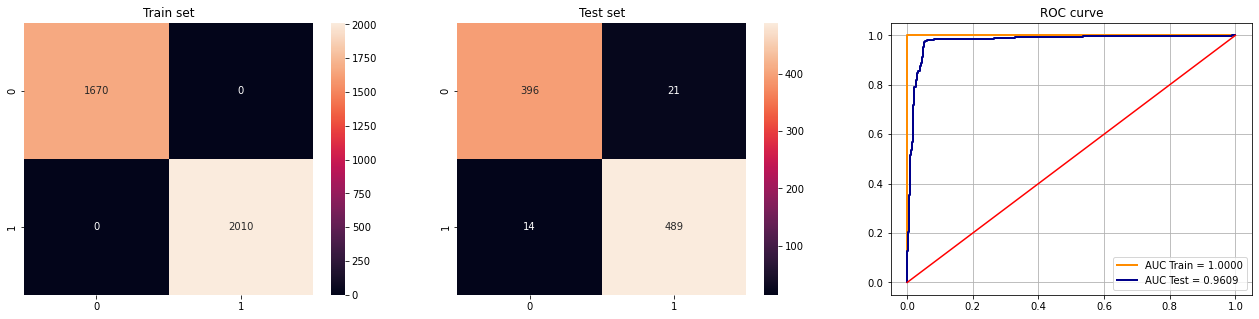
\includegraphics[width=\linewidth]{chapters/deteccion/images/lr.png}
        \caption{Métricas para el modelo logístico}
        \label{fig.lr}
  \end{figure}
  
  En la Tabla \ref{tabla.lr} se detallan las métricas derivadas de la matriz de confusión. 

\begin{table}[H]
\centering
\begin{tabular}{|c|c|c|c|c|c|}
\hline
      & Accuracy & Precision & Recall & AUC    & $F_1$ score \\ \hline
Train & 1.0   & 1.0    & 1.0 & 1.0 & 1.0      \\ \hline
Test  & 0.962      & 0.9588    & 0.9722 & 0.9609  & 0.9654      \\ \hline
\end{tabular}
\caption{Métricas para el modelo logístico}
\label{tabla.lr}
\end{table}


\subsection{Decision tree}

Luego del entrenamiento se obtuvieron la matriz de confusión y curva roc tanto para train como para test, las cuales son mostradas en la Fig. \ref{fig.dt}. 

\begin{figure}[H]
\centering
        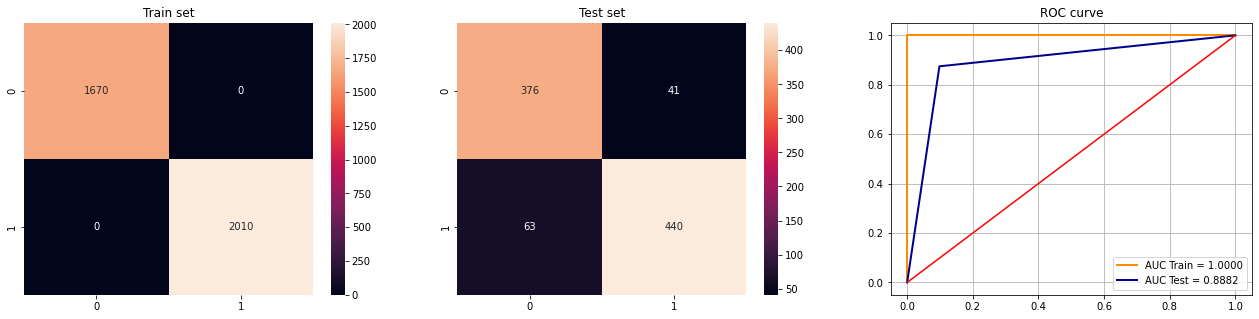
\includegraphics[width=\linewidth]{chapters/deteccion/images/dt.png}
        \caption{Métricas para el modelo de árbol de decisión}
        \label{fig.dt}
  \end{figure}
  
  En la Tabla \ref{tabla.dt} se detallan las métricas derivadas de la matriz de confusión. 

\begin{table}[H]
\centering
\begin{tabular}{|c|c|c|c|c|c|}
\hline
      & Accuracy & Precision & Recall & AUC    & $F_1$ score \\ \hline
Train & 1.0   & 1.0    & 1.0 & 1.0 & 1.0      \\ \hline
Test  & 0.887      & 0.9148    & 0.8748 & 0.8882  & 0.8943      \\ \hline
\end{tabular}
\caption{Métricas para el modelo de árbol de decisión}
\label{tabla.dt}
\end{table}

Comparando las métricas obtenidas para los conjuntos de entrenamiento y prueba, se evidencia claramente que el modelo sufre de sobreajuste. Aunque se podría haber intentado mitigar este sobreajuste mediante la optimización de hiperparámetros, se descartó esta opción debido a la disponibilidad de un modelo superior (random forest) y al considerable aumento en el tiempo de ajuste de dicho modelo.

\subsection{KNN}

Luego del entrenamiento se obtuvieron la matriz de confusión y curva roc tanto para train como para test, las cuales son mostradas en la Fig. \ref{fig.knn}. 

\begin{figure}[H]
\centering
        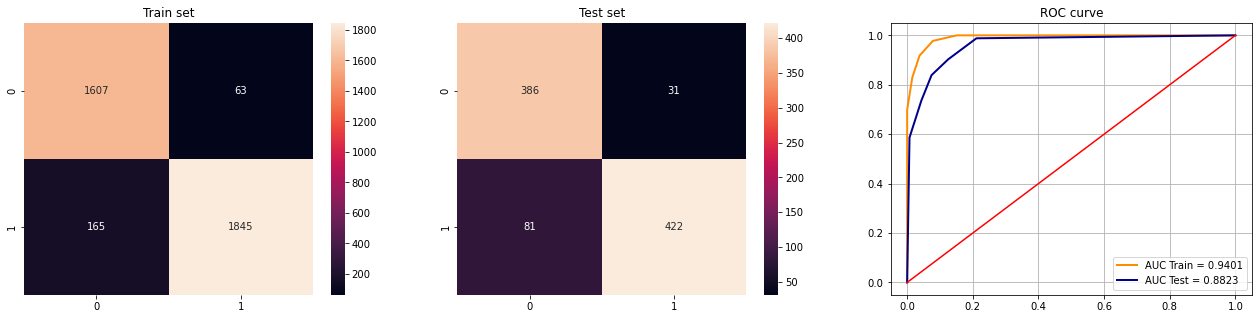
\includegraphics[width=\linewidth]{chapters/deteccion/images/knn.png}
        \caption{Métricas para el modelo KNN}
        \label{fig.knn}
  \end{figure}
  
  En la Tabla \ref{tabla.knn} se detallan las métricas derivadas de la matriz de confusión. 

\begin{table}[H]
\centering
\begin{tabular}{|c|c|c|c|c|c|}
\hline
      & Accuracy & Precision & Recall & AUC    & $F_1$ score \\ \hline
Train & 1.0   & 1.0    & 1.0 & 1.0 & 1.0      \\ \hline
Test  & 0.887      & 0.9148    & 0.8748 & 0.8882  & 0.8943      \\ \hline
\end{tabular}
\caption{Métricas para el modelo KNN}
\label{tabla.knn}
\end{table}


\subsection{Red neuronal convolucional}

Finalmente se aplicó un modelo de $\textit{deep learning}$, una red neuronal convolucional. Básicamente consta de cuatro bloques $\textit{convolucional}$, $\textit{batch normalization}$, $\textit{max pooling}$, una capa de $\textit{flatten}$ y luego tres bloques de capa $\textit{densa y dropout}$ como regularización. El optimizador utilizado fue $\textit{adam}$, la función de pérdida $\textit{binary crossentropy}$ tomando como métrica $\textit{accuracy}$ dado que el dataset estaba razonablemente balanceado. Se entrenó la red con un $\textit{batch size}$ de 10, $\textit{validation split}$ de 0.2 y con 100 $\textit{epochs}$.

Antes de calcular las métricas correspondientes de clasificación para este modelo, se procedió a investigar si hubo un overfitting durante el entrenamiento. Para esto se graficó la función de pérdida y el accuracy tanto de train como de test para cada epoch. La gráfica se muestra en la Fig. \ref{fig.loss}. 


\begin{figure}[H]
\centering
        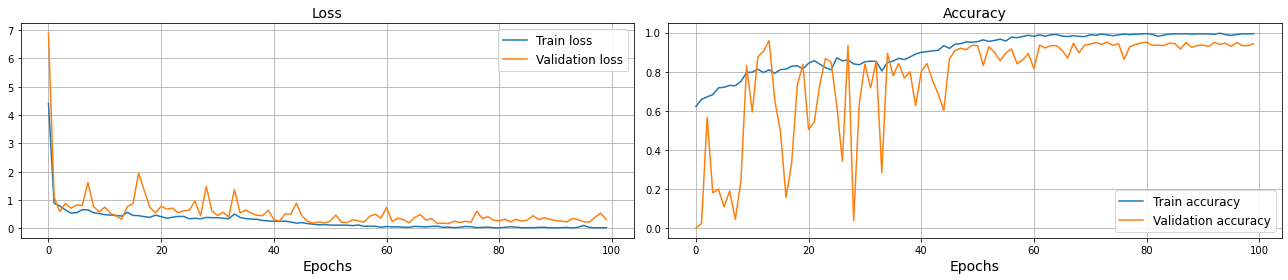
\includegraphics[width=\linewidth]{chapters/deteccion/images/loss.png}
        \caption{Función de pérdida y accuracy para el modelo de red convolucional.}
        \label{fig.loss}
  \end{figure}

Se observa que en principio no hay un overfitting. Al momento de calcular las predicciones, el modelo entrega una probabilidad de pertenecer a cada clase, por lo tanto se eligió un valor de umbral, el cual fue de 0.59, es decir, aquellas probabilidades mayores a 0.59 serían clasificadas como 1, es decir, con tumor y viceversa. El detalle de estos cálculos se encuentra en el código disponible en el Github. Una vez teniendo este valor umbral se calcularon las métricas, las cuales se muestran en la Tabla \ref{tabla.cnn} y en la Fig. \ref{fig.cnn_me}.


\begin{figure}[H]
\centering
        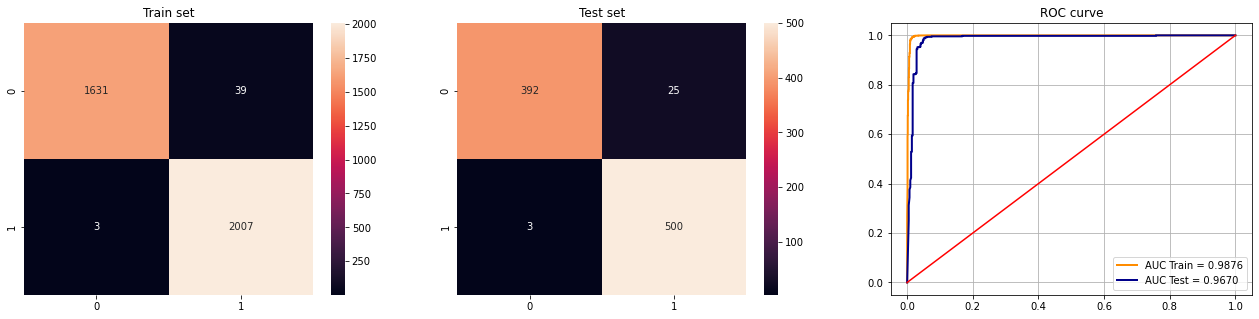
\includegraphics[width=\linewidth]{chapters/deteccion/images/cnn_met.png}
        \caption{Métricas para el modelo de red convolucional}
        \label{fig.cnn_me}
  \end{figure}

\begin{table}[H]
\centering
\begin{tabular}{|c|c|c|c|c|c|}
\hline
      & Accuracy & Precision & Recall & AUC    & $F_1$ score \\ \hline
Train & 0.9886   & 0.9809    & 0.9985 & 0.9876 & 0.9896      \\ \hline
Test  & 0.9696      & 0.9524    & 0.994 & 0.967  & 0.9728      \\ \hline
\end{tabular}
\caption{Métricas para el modelo de red convolucional}
\label{tabla.cnn}
\end{table}

\section{Resumen de modelos}

En términos de métricas, el mejor modelo pareciera ser el Random Forest, sin embargo, considero que el de red neuronal convolucional es mejor porque exhibe un mejor recall. 

En el contexto del problema, es importante no solo clasificar correctamente a los verdaderos positivos (pacientes efectivamente con tumores), sino también reducir los falsos negativos (pacientes con tumor pero clasificados como sanos).

Por este motivo, se optó por el modelo de redes neuronales convolucionales.









